\section{Basics}
\begin{frame}
\frametitle{An introduction to control}
\end{frame}

\subsection[Classical control loop]{Classical control loop}
\begin{frame}
\frametitle{What is control?}
\begin{itemize}
	\item The goal is to find an input (control signal U(s)) such that the process $P(s)$ produces the desired output
	\item Open loop control system: the actual output signal $Y(s)$ has no effect on the control action
\end{itemize}
\vspace{-1em}
\begin{figure}
	\centering
	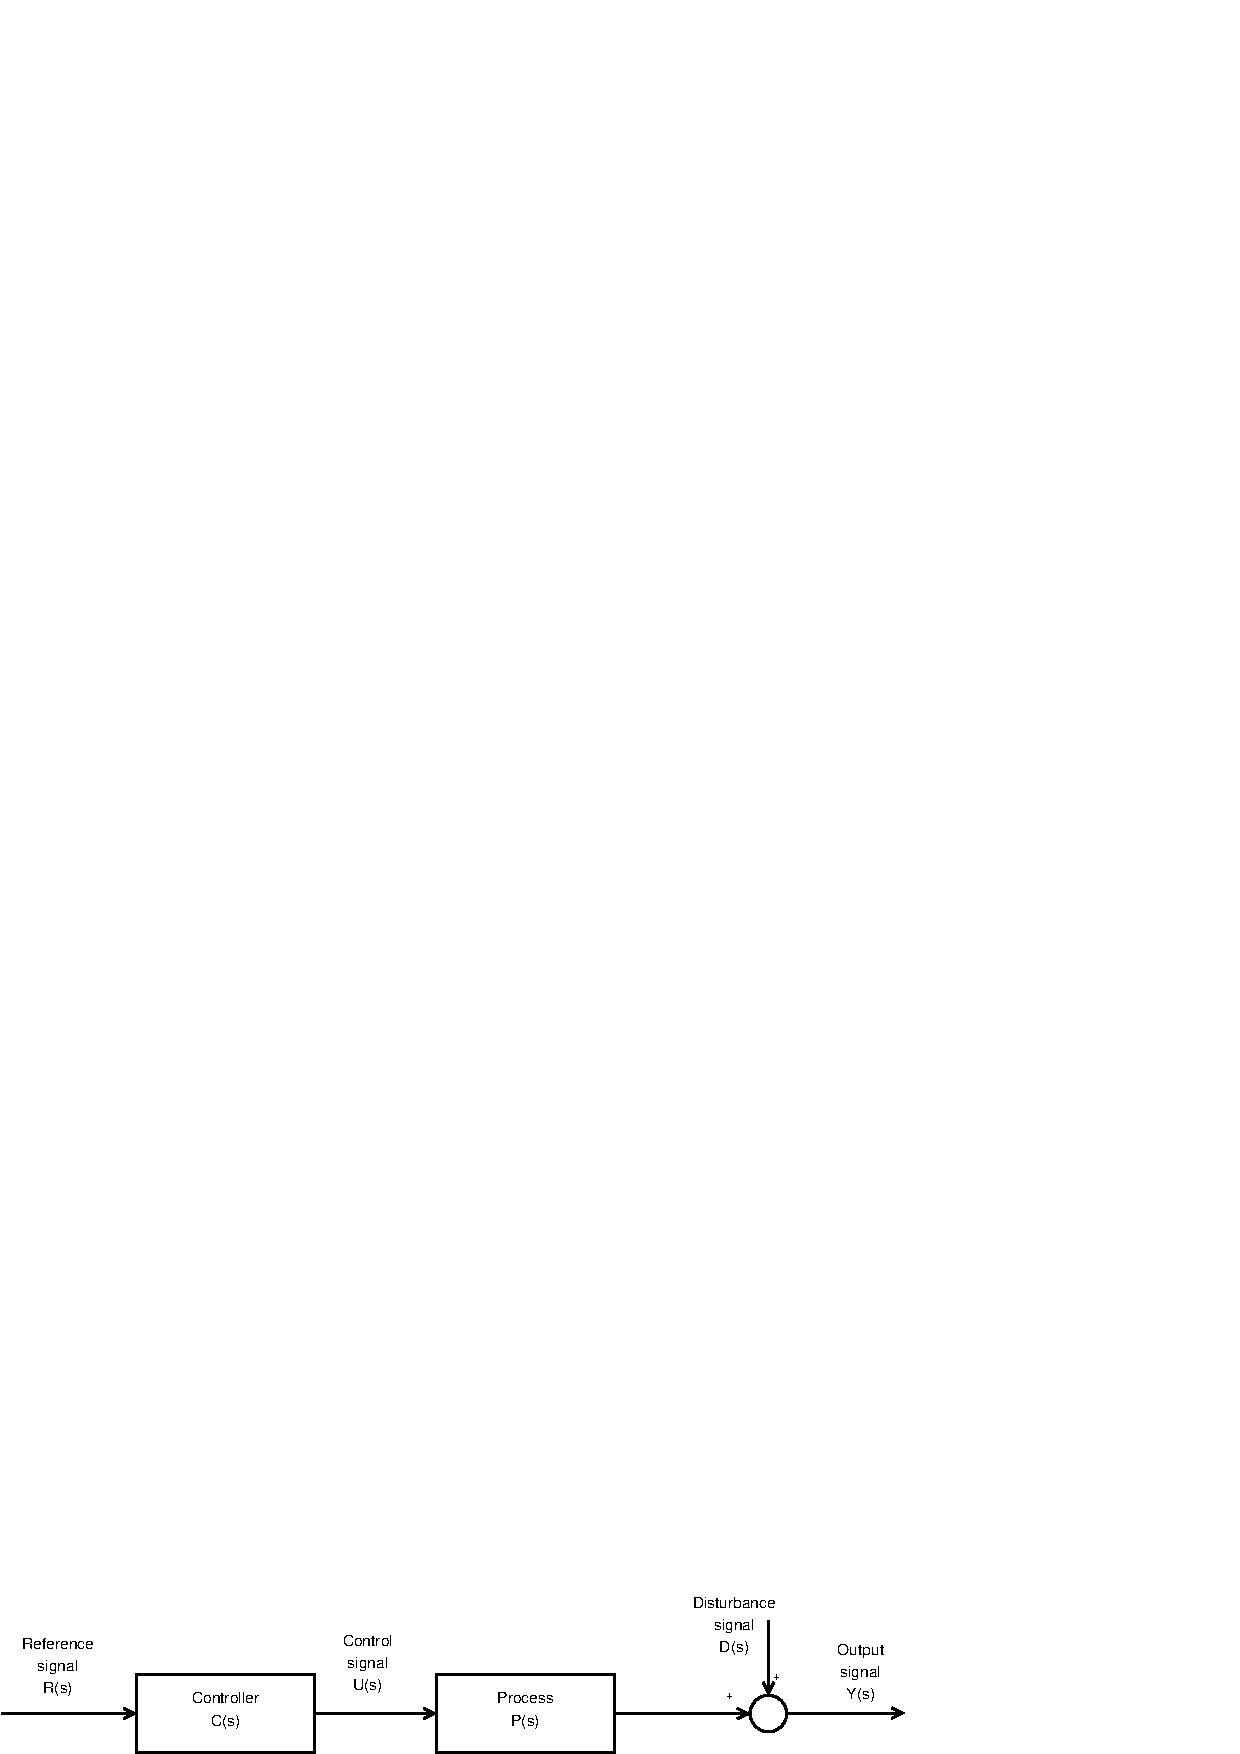
\includegraphics[width=0.8\linewidth]{Open-Loop}
	\label{fig:Open-Loop}
\end{figure}
\begin{align*}
	Y(s) = P(s)U(s) = P(s)C(s)R(s) \\
\end{align*}
Remember the example of pouring a glass of water without looking at the glass
\end{frame}

\begin{frame}
	\frametitle{A general set-up of a closed loop system}
	\vspace*{-1em}
	\begin{itemize}
		\item We will focus on \underline{closed loop control systems}
		\begin{figure}
\centering
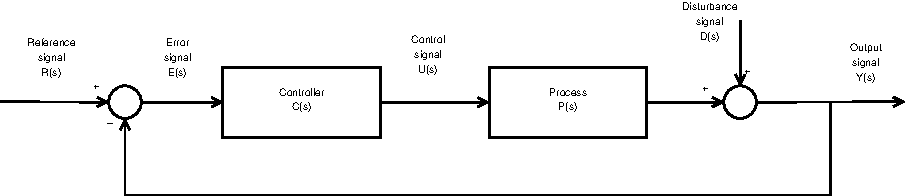
\includegraphics[width=0.7\linewidth]{Closed-Loop}
\label{fig:Closed-Loop}
\end{figure}
\item Example: \href{http://homes.esat.kuleuven.be/~magudelo/_html5/test11.html}{\underline{Inverted pendulum}}

\item Digital Control Loop:
\begin{figure}
\centering
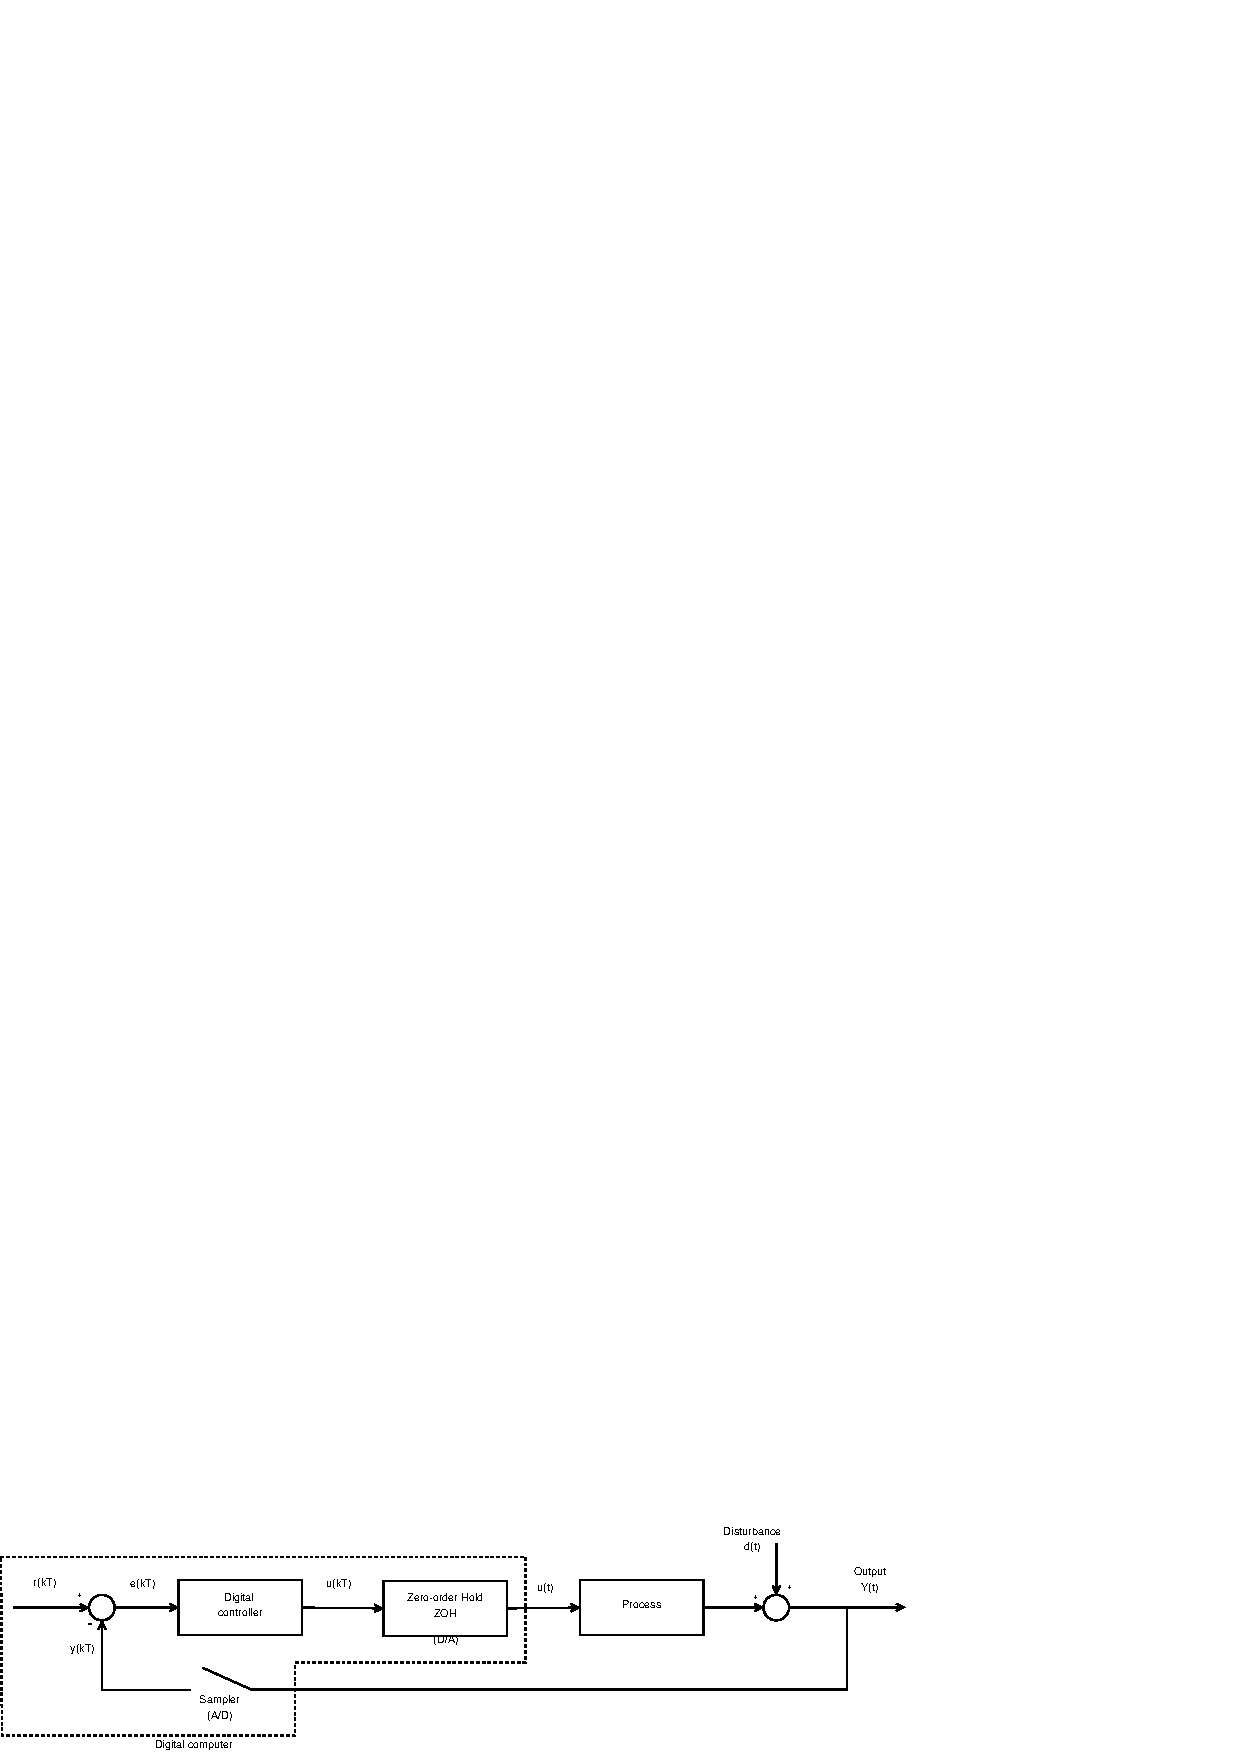
\includegraphics[width=0.6\linewidth]{digital-control-system}
\label{fig:digital-control-system}
\end{figure}

	\end{itemize}
\end{frame}

\subsection[Demo: Inverted Pendulum]{Demo: Inverted Pendulum}
\begin{frame}
	\begin{figure}
\centering
\includegraphics[width=0.7\linewidth]{"Inverted Pendulum"}
\caption{\href{http://homes.esat.kuleuven.be/~magudelo/_html5/test11.html}{{Inverted Pendulum}}}
\label{fig:InvertedPendulum}
\end{figure}
\end{frame}

\subsection[Elements]{Elements}
\begin{frame}
	\frametitle{Concrete Controllers}
	\begin{itemize}
		\item On-off controller
		\begin{itemize}
			\item Thermostate at home
		\end{itemize}
		\item \textbf{PID controllers, Lead and lag compensators (this course)}
		\begin{itemize}
			\item Cruise-control in your car
		\end{itemize}
		\item More advanced controllers
		\begin{itemize}
			\item STATE-space feedback controllers
			\item Model Predictive Controller (MPC)
			\item Fuzzy Control
			\item Neuro-fuzzy Control
			\item ...
		\end{itemize}
	\end{itemize}
\end{frame}


\section{Control Goals}
\begin{frame}
	\frametitle{What is good control?}
	\begin{itemize}
		\item Before we will start to design control systems we will first focus on the question. What is good control?
		\item It depends on the application
		\begin{itemize}
			\item Stability
			\item Disturbance rejection
			\item Reference tracking (speed)
			\item Sensitivity to errors on model
			\item Etc...
		\end{itemize}
	\end{itemize}
\end{frame}

\subsection[stability]{stability}
\begin{frame}
	\frametitle{Examples: stability}
\begin{figure}
\centering
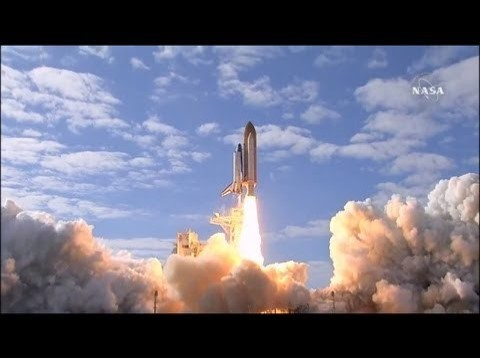
\includegraphics[width=0.7\linewidth]{shuttle}
\caption{Space shuttles are like inverted pendulums. How do you make sure they don't flip over.}
\label{fig:shuttle}
\end{figure}
\end{frame}

\subsection[disturbance rejection]{disturbance rejection}
\begin{frame}
	\frametitle{Examples: Disturbance rejection}
	\begin{itemize}
		\item Your body will try to keep the temperature in your body as constant as possible. No matter what the outside temperature is. Two people will have almost the same body temperature.
	\end{itemize}
	\begin{figure}
\centering
\begin{minipage}{0.45\textwidth}
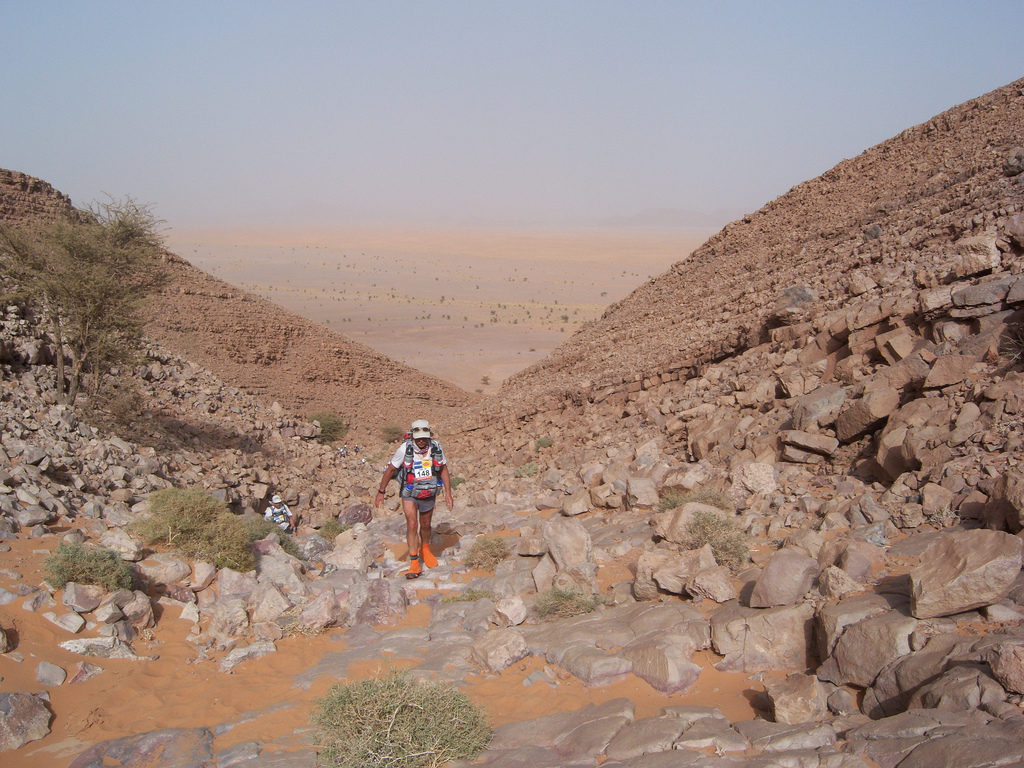
\includegraphics[width=0.7\linewidth]{marathon-des-sables}
\caption{Flickr.com, \underline{tent86}, Marathon Des Sables 046}
\label{fig:marathon-des-sables}
\end{minipage}
\centering
\begin{minipage}{0.45\textwidth}
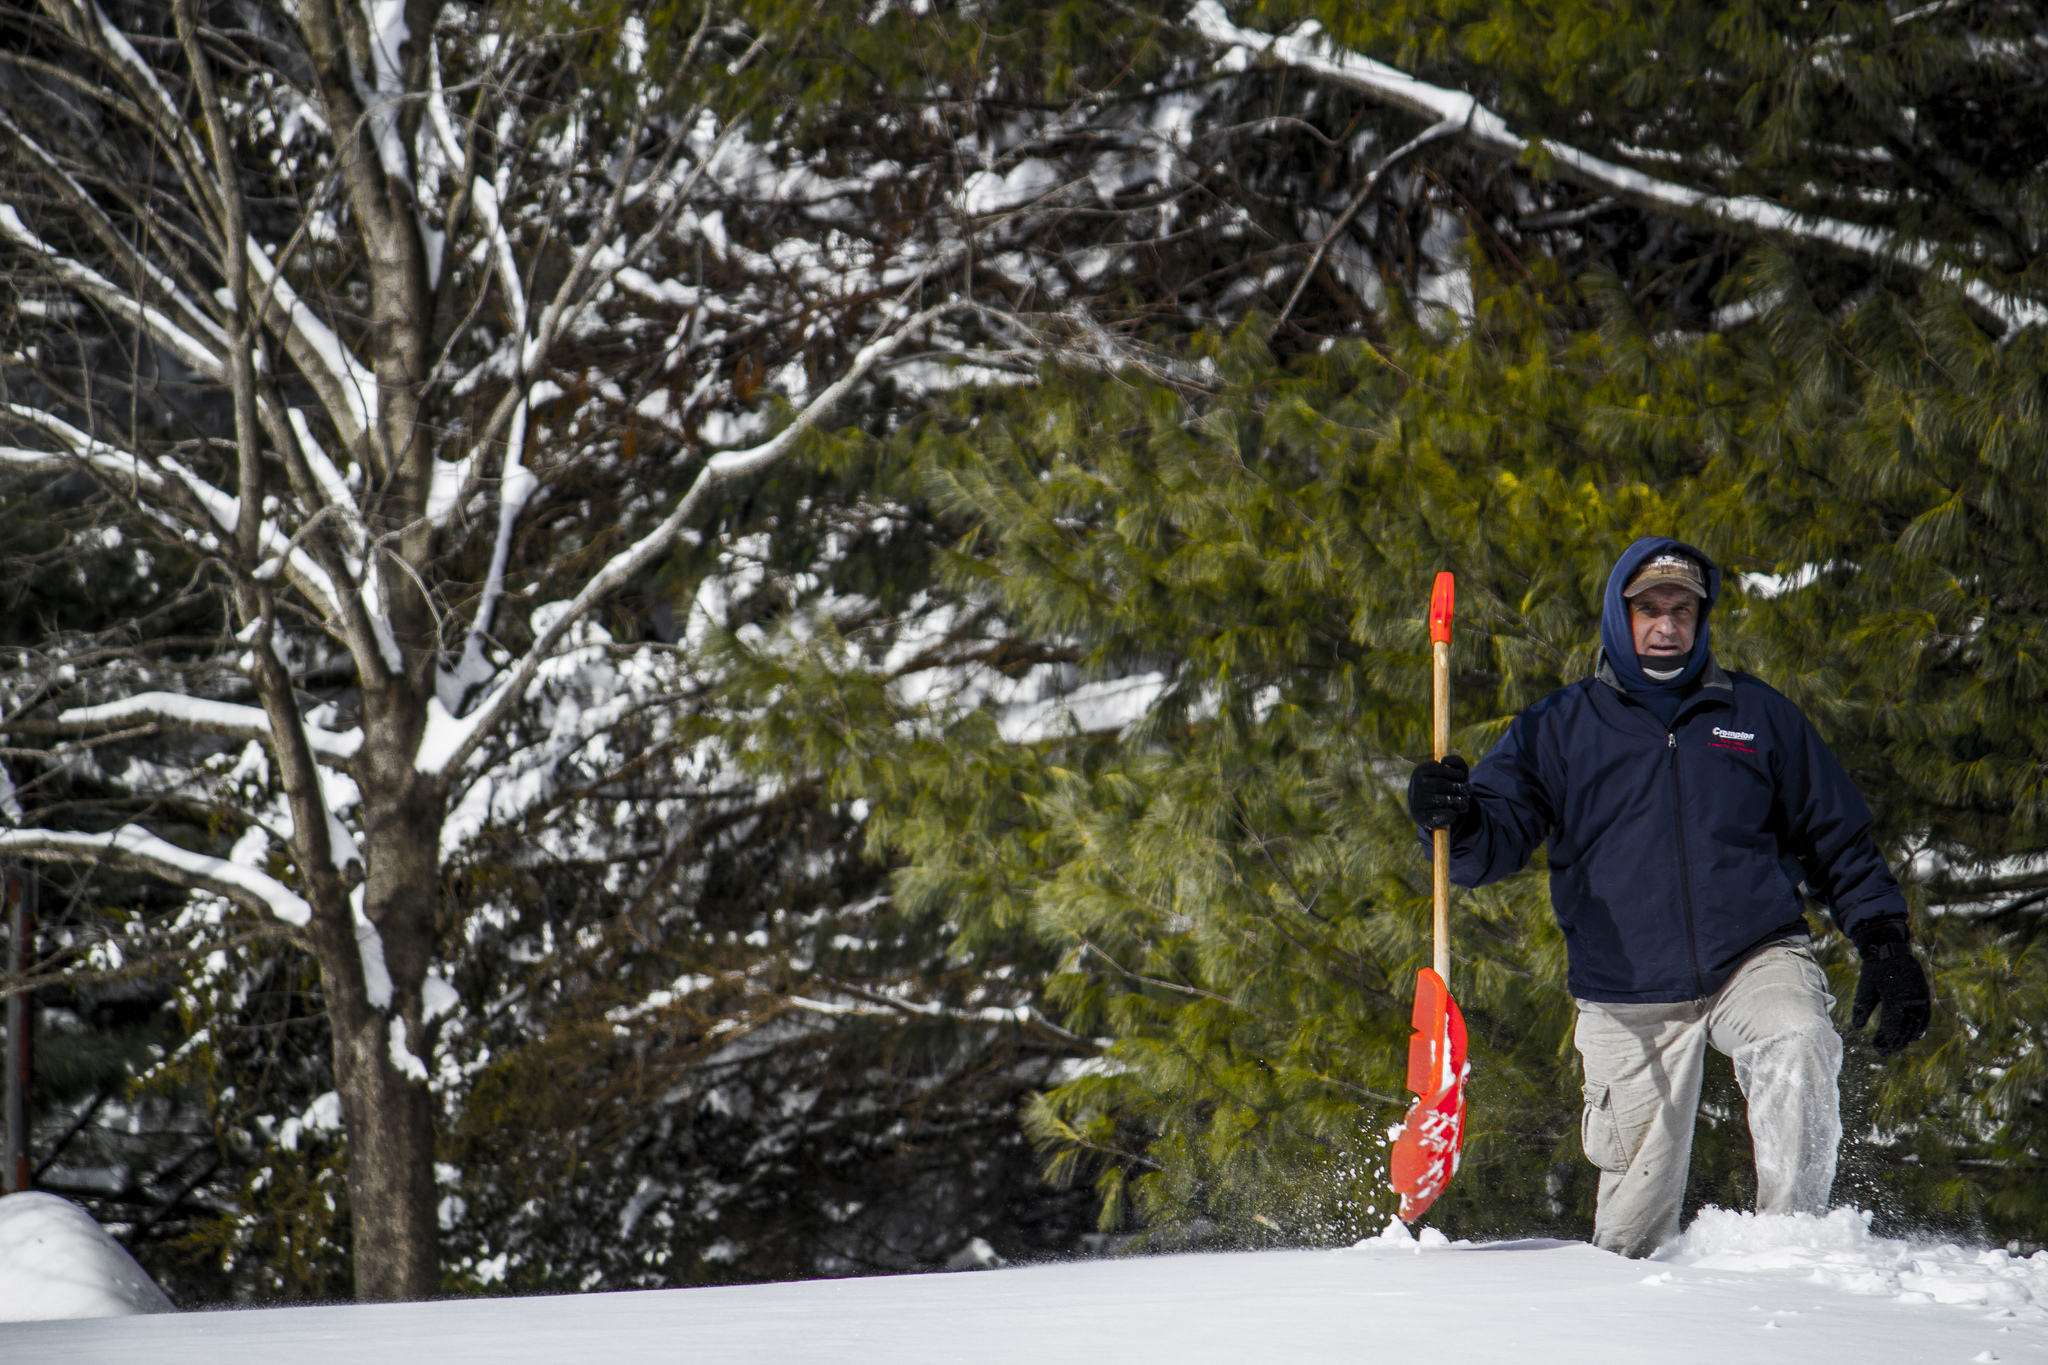
\includegraphics[width=0.7\linewidth]{enduring}
\caption{\underline{Jack Zalium,} Enduring, https://creativecommons.org/licenses/by-nd/2.0/}
\label{fig:enduring}
\end{minipage}
\end{figure}

\end{frame}

\subsection[Tracking]{Reference tracking}
\begin{frame}
	\frametitle{Examples: Reference tracking}
	\begin{figure}
\centering
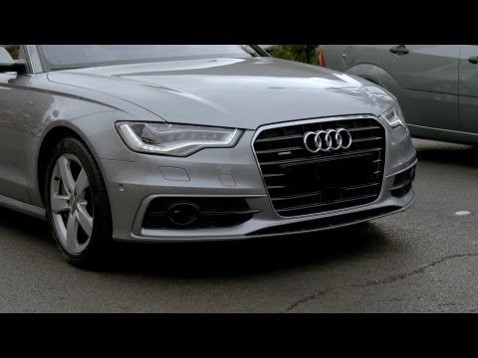
\includegraphics[width=0.7\linewidth]{audi-tracking}
\caption{Audi has a system for automatic driving in traffic jams. The audi will follow the car in front of him at an appropriate distance. \href[pdfnewwindow=true]{https://www.youtube.com/watch?v=Qa_ZSRj0WM0}{\nolinkurl{https://www.youtube.com/watch?v=Qa_ZSRj0WM0}}}
\label{fig:audi-tracking}
\end{figure}
\end{frame}

\subsection[Exercise]{Exercise}
\begin{frame}
	\frametitle{Exercise: name the correct property}
	\begin{figure}
\centering
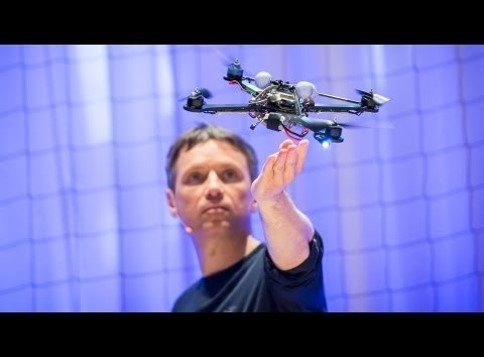
\includegraphics[width=0.7\linewidth]{ted-drone}
\label{fig:ted-drone}
\end{figure}

\end{frame}


\section{Closed-loop system}

\begin{frame}
	\frametitle{Transfer function of a closed-loop system}
	\vspace*{-1.5em}
	{\small
	\begin{flalign*}
		Y(s) - D(s) &= P(s)U(s) \\
		& \text{with } U(s) = C(s)E(s) \\
		Y(s) - D(s) &= P(s)C(s)E(s) \\
		& \text{with } E(s) = R(s) - Y(s) \\
		Y(s) - D(s) &= P(s)C(s) (R(s) - Y(s)) \\
		Y(s) - D(s) &= P(s)C(s)R(s) - P(s)C(s)Y(s) \\
		&\Rightarrow Y(s) = \frac{P(s)C(s)}{1 + P(s)C(s)}R(s) + \frac{1}{1 + P(s)C(s)}D(s)
	\end{flalign*}
	} %
	\vspace*{-1.5em}
	\begin{figure}
\centering
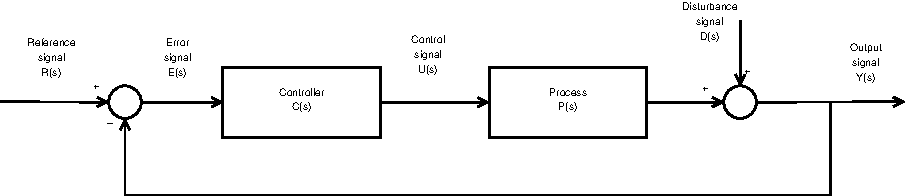
\includegraphics[width=0.7\linewidth]{Closed-Loop}
\label{fig:Closed-Loop2}
\end{figure}

\end{frame}


\begin{frame}
	\frametitle{Transfer function from $R(s)$ to $Y(s)$}
	We define S as the transfer function from $R(s)$ to $Y(s)$
	\begin{align*}
	S(s) \triangleq \frac{P(s)C(s)}{1 + P(s) C(s)}
	\end{align*}
	This transfer function $S(s)$ will help us to evaluate tracking
	
	Almost perfect tracking: the output $Y(s)$ will follow $R(s)$ very closely $\Rightarrow S(s) \approx 1$
	
\end{frame}


\begin{frame}
	\frametitle{Transfer function from $D(s)$ to $Y(s)$}
	We define $T(s)$ as the transfer function from $D(s)$ to $Y(s)$.
	\begin{align*}
	T(s) \triangleq \frac{1}{1 + P(s)C(s)}
	\end{align*}
	If the disturbance rejection is very good the disturbances will have almost no effect on the output $\Rightarrow T \approx 0$ \\
	
	\[
	\begin{cases}
		\left| S(j\omega) \right| \cong 1 \\
		\left| T(j\omega) \right| \cong 0
	\end{cases}
	\]
	$\Rightarrow  \left| P(j\omega)C(j\omega) \right|$ \textbf{(open loop gain)} is very large. \\
	
	! a large open loop amplification might lead to an unstable system
	
\end{frame}

\begin{frame}
	\frametitle{Example: Which controller do you prefer}
	The transfer function from $R(s)$ to $Y(s)$ for two different controllers for high precision surgery\\
	\begin{minipage}{0.7\linewidth}
	\begin{figure}
\centering
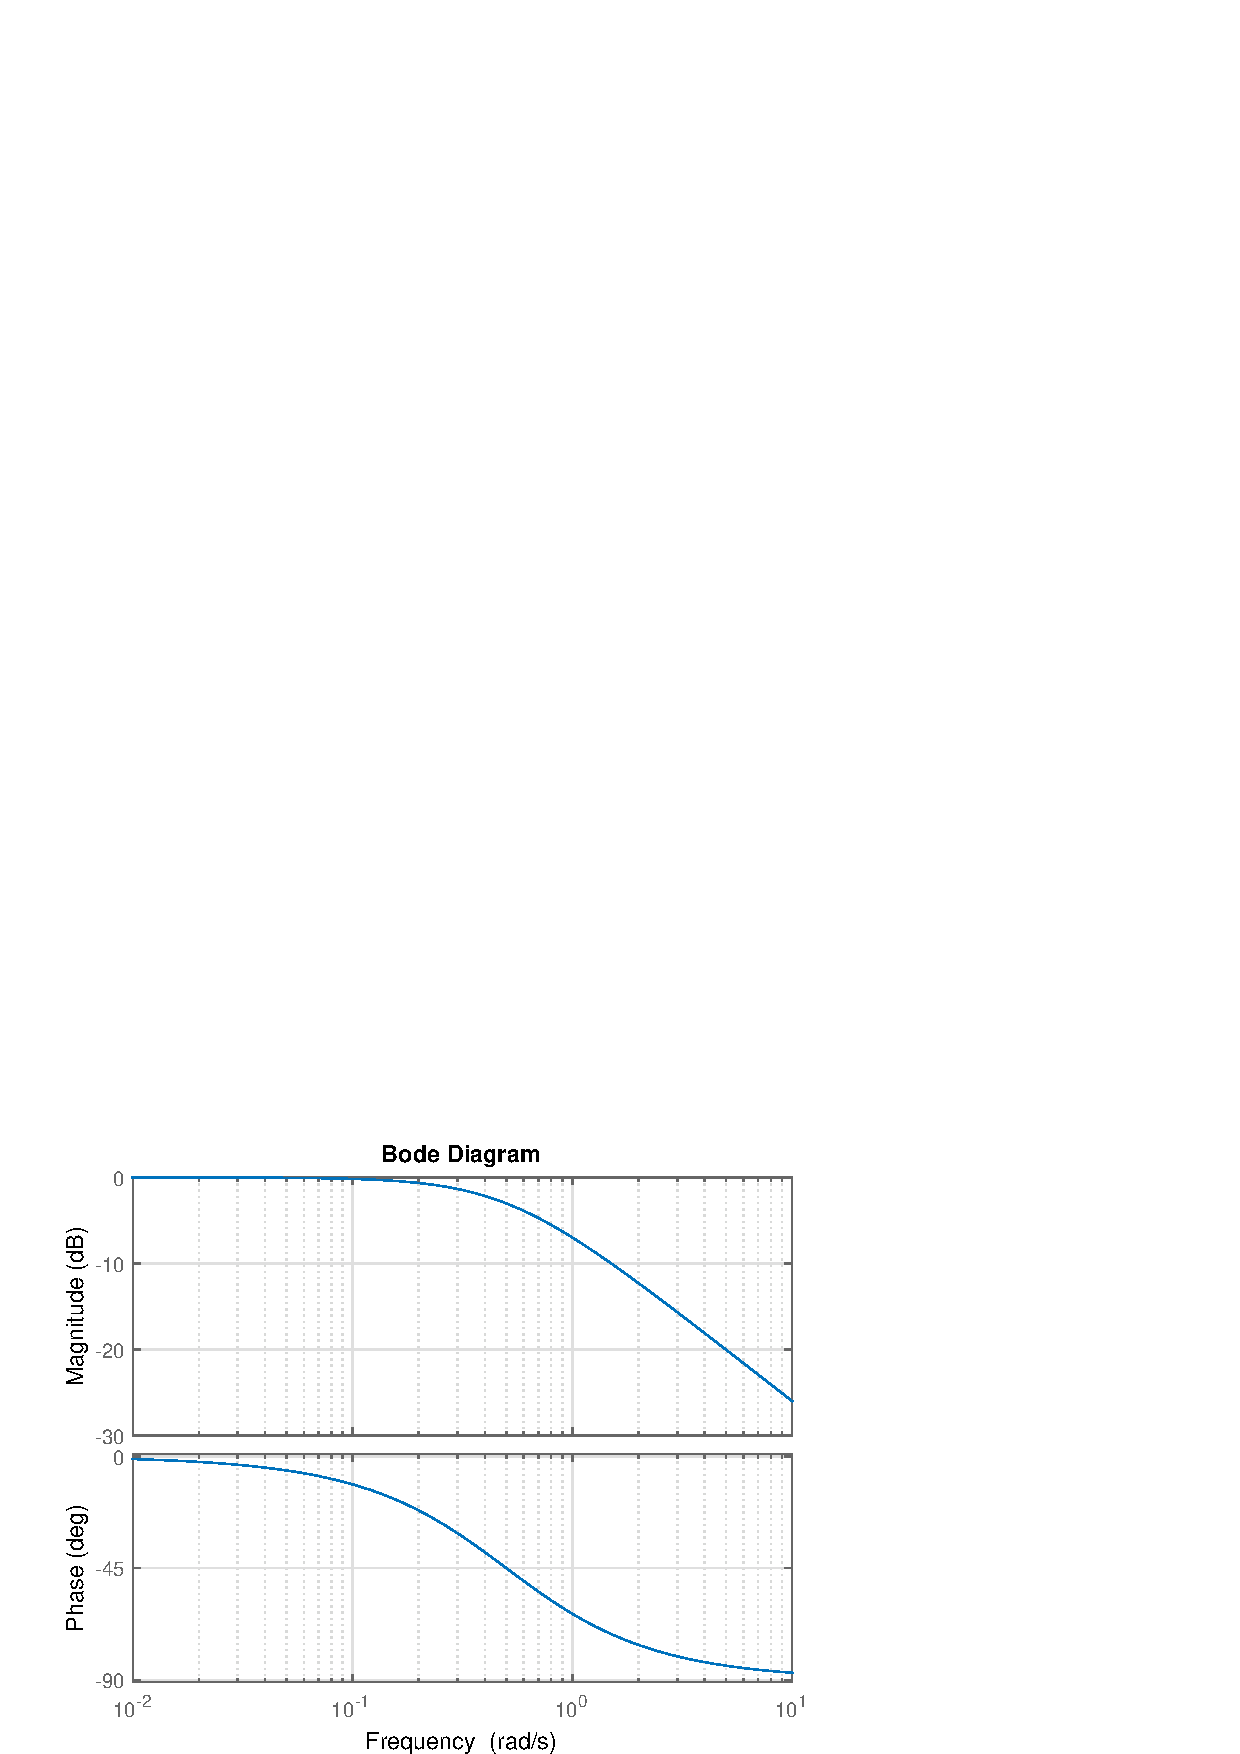
\includegraphics[width=\columnwidth,height=6em]{smooth-bode}
\label{fig:smooth-bode}
\end{figure}
\end{minipage}
\hfill
\begin{minipage}{0.2\linewidth}
	\[\frac{0.5}{s+0.5}\]
\end{minipage}
\vspace*{-3em}
\begin{minipage}{0.7\linewidth}
\begin{figure}
\centering
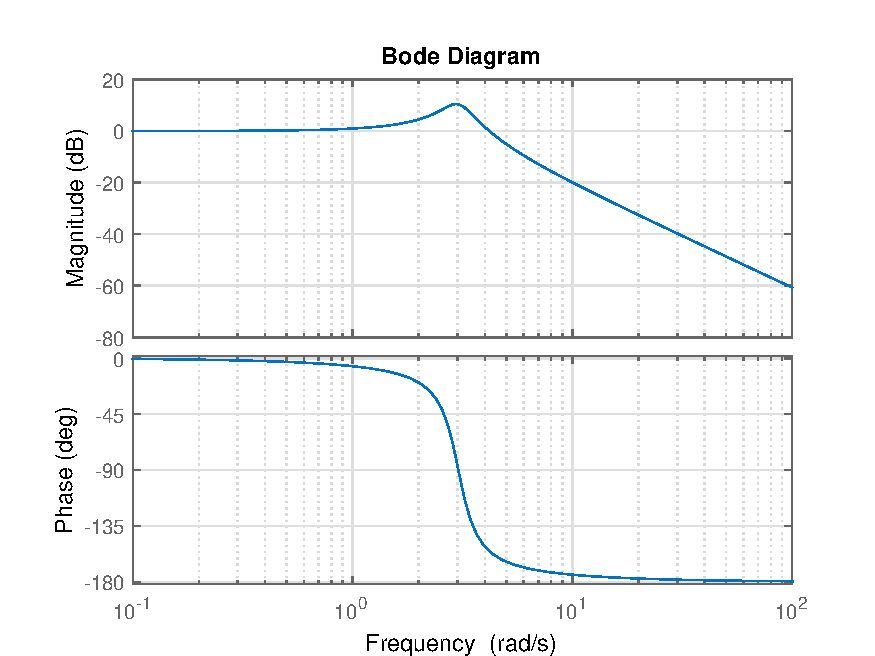
\includegraphics[width=\columnwidth,height=6em]{osc-bode}
\label{fig:osc-bode}
\end{figure}
\end{minipage}
\hfill
\begin{minipage}{0.2\linewidth}
	\[\frac{10}{1.09s^2 + s + 10}\]
\end{minipage}
\end{frame}


\begin{frame}
	\frametitle{Example: step response of both controllers}
	The ouput $Y(s)$ when $R(s)$ is a step function.
	\vspace*{-1em}
	\begin{figure}
\centering
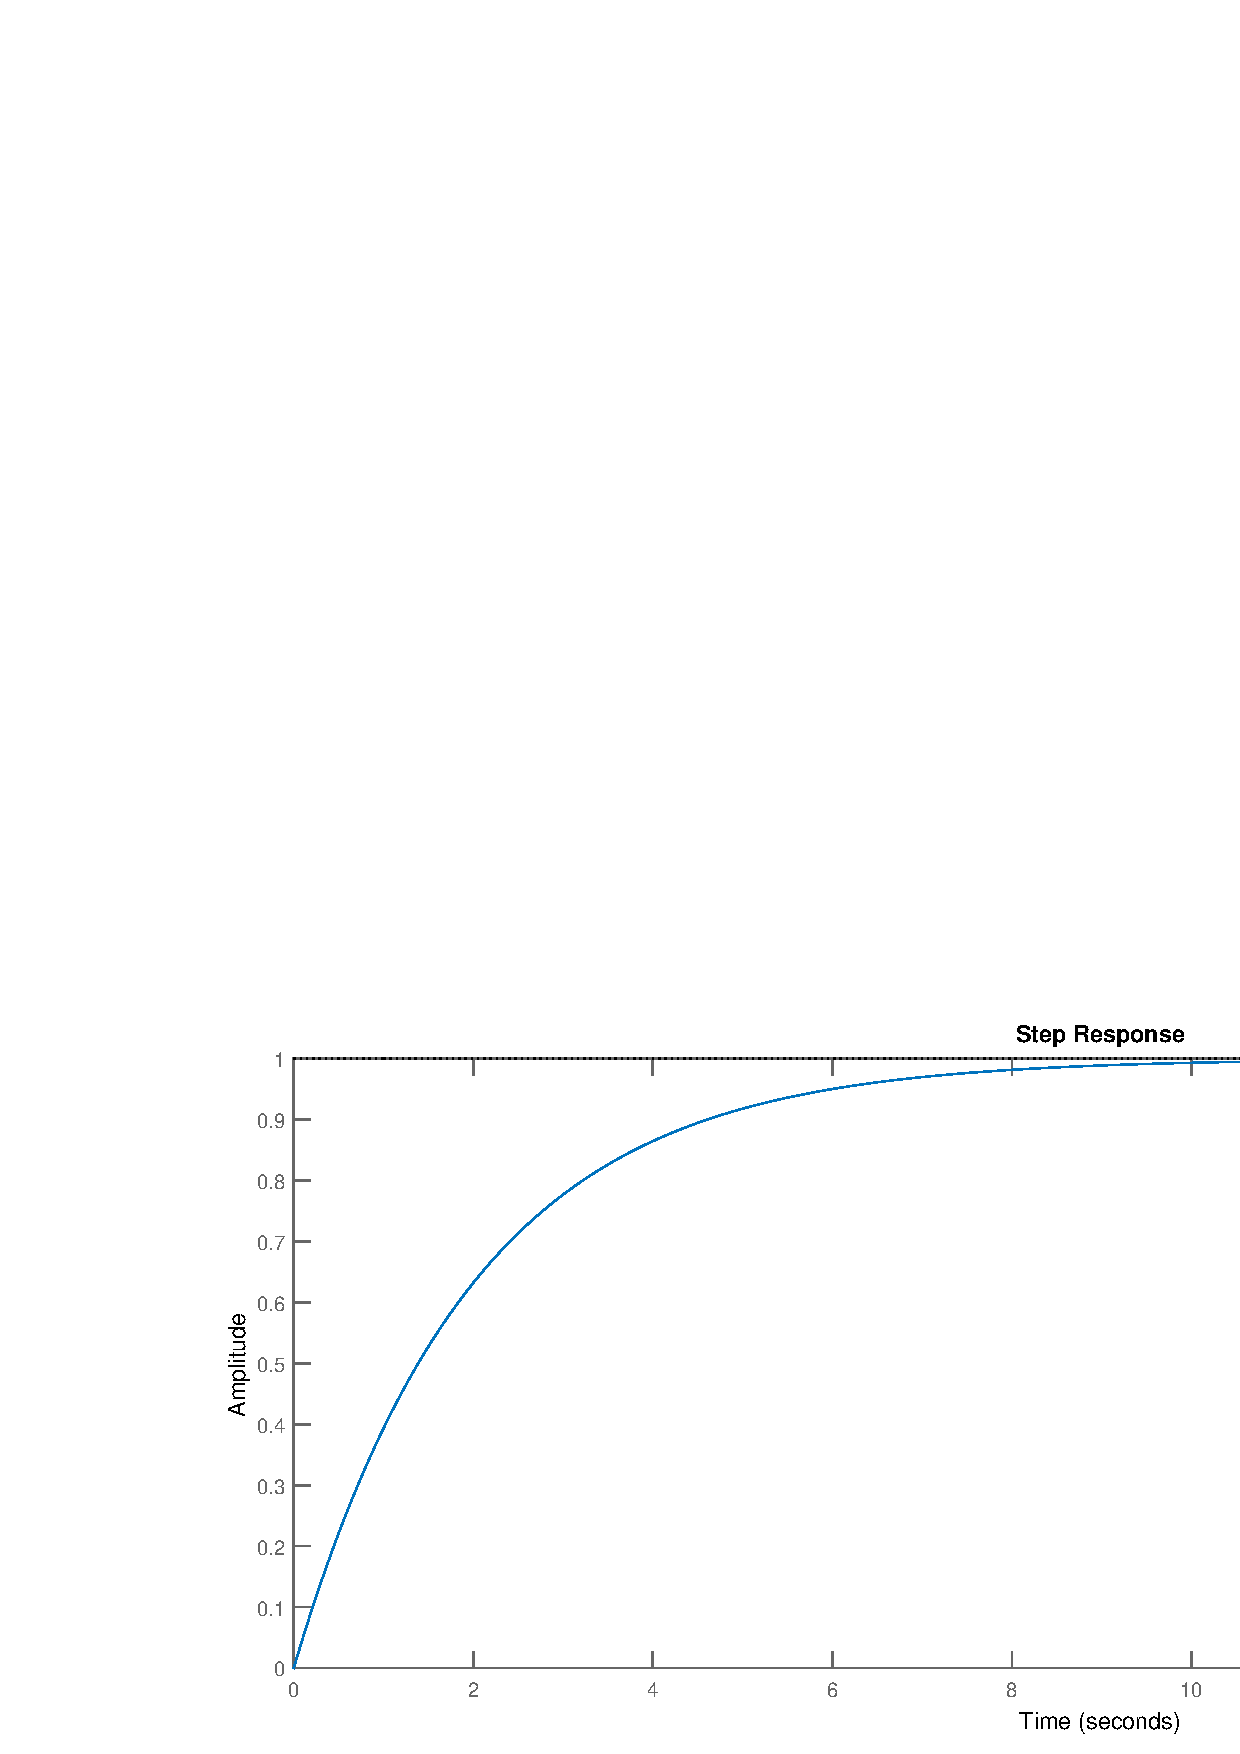
\includegraphics[width=\columnwidth,height=8em]{smooth-step}
\label{fig:smooth-step}
\end{figure}
\vspace*{-3em}
\begin{figure}
\centering
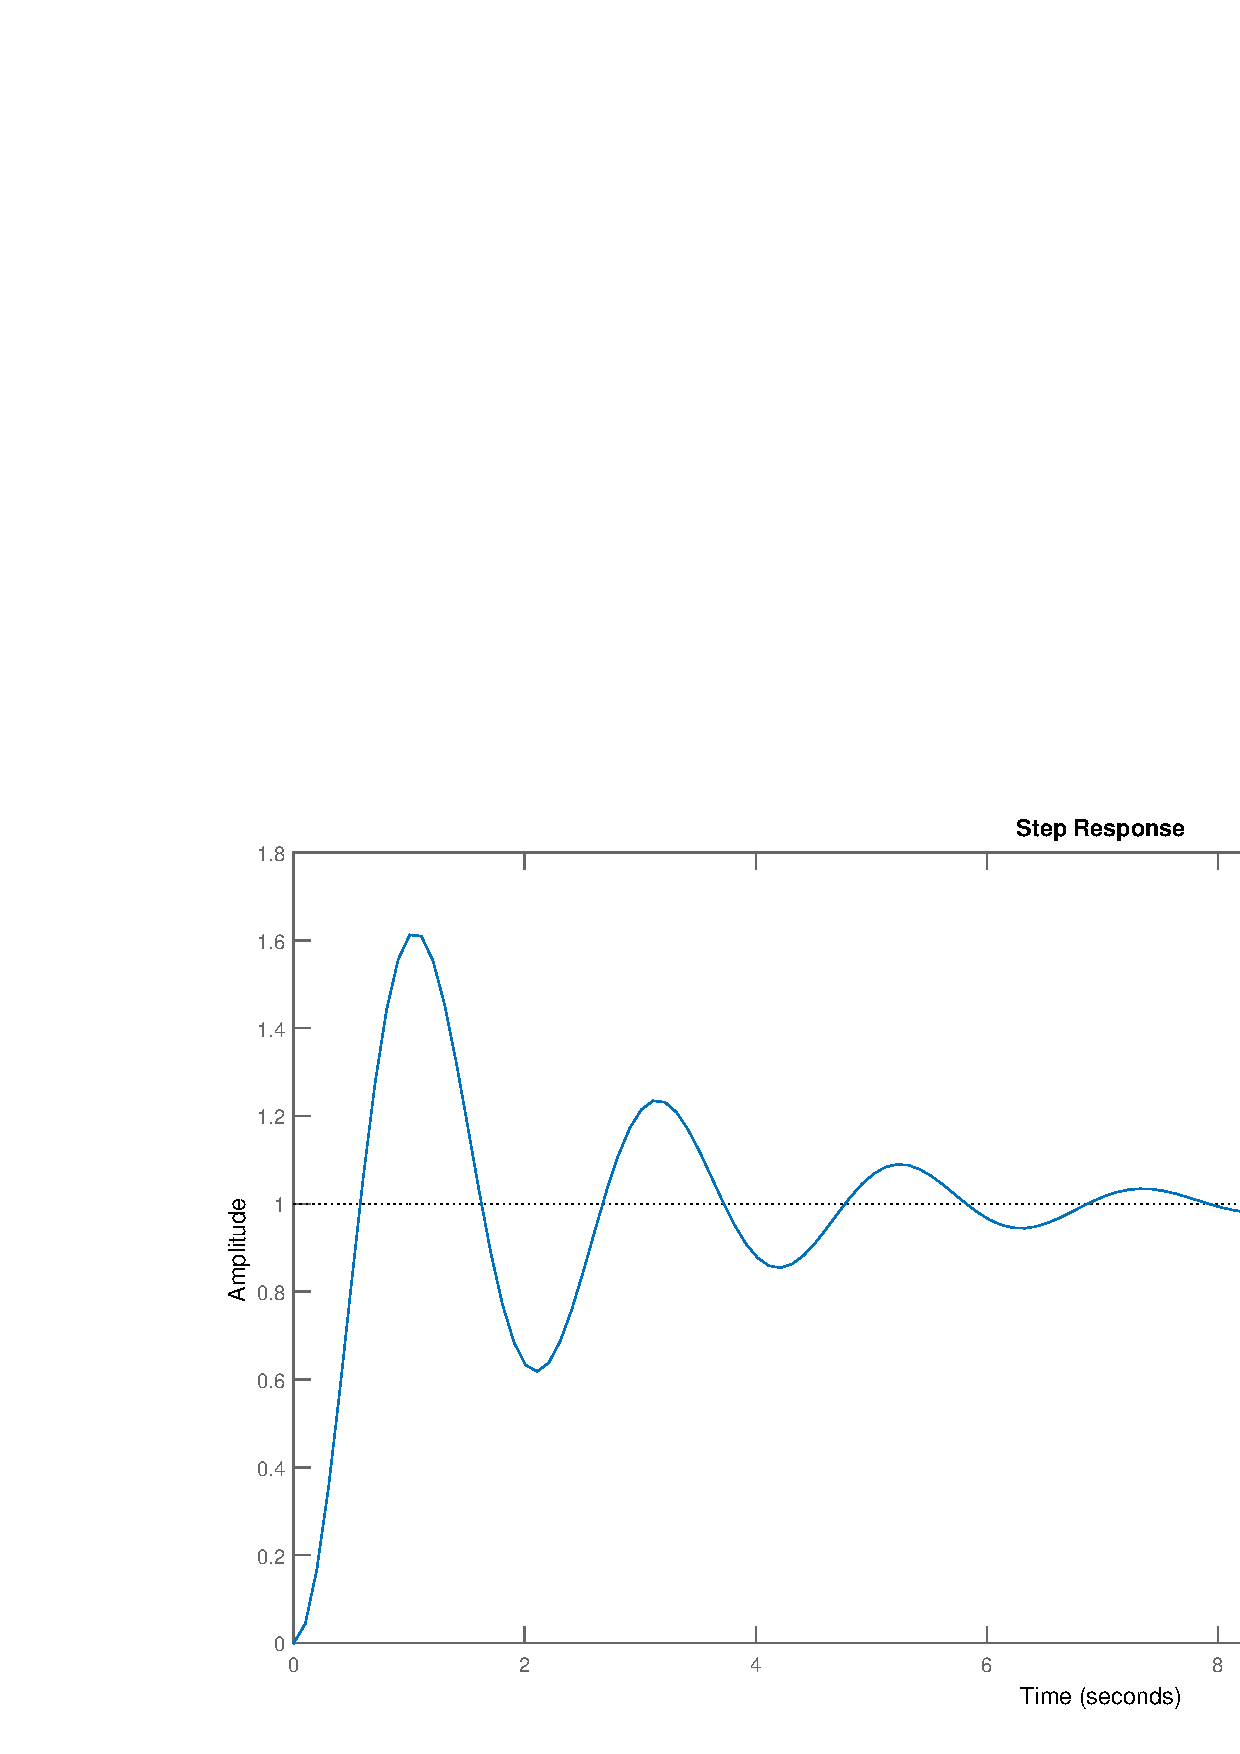
\includegraphics[width=\columnwidth,height=8em]{osc-step}
\label{fig:osc-step}
\end{figure}

\end{frame}

\begin{frame}
	\frametitle{Quality of reference tracking}
	\begin{minipage}{0.5\linewidth}
		\begin{itemize}
			\item Look at the step response from $R(s)$ to $Y(s)$. All the known criteria can help you determine the quality.
			\begin{itemize}
				\item Rise-time
				\item Settling time
				\item Steady state error
				\item Overshoot
				\item ...
			\end{itemize}
		\end{itemize}
	\end{minipage}
	\hfill
	\begin{minipage}{0.4\linewidth}
		\begin{figure}
			\centering
			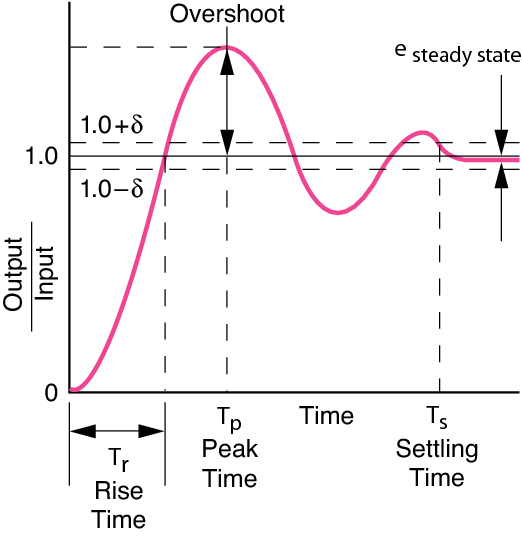
\includegraphics[width=1\linewidth]{properties}
			\label{fig:properties}
			\caption{\tiny \raggedleft
				\href{http://www.newport.com/Control-Theory-Terminology/178319/1033/content.aspx}{\nolinkurl{http://www.newport.com/Control-Theory-Terminology/178319/1033/content.aspx}}}
		\end{figure}
	\end{minipage}
\end{frame}

\begin{frame}
	\frametitle{Model errors}
	\begin{itemize}
		\item In practice, the transfer function $P(S)$ is often unknown. It is important to know how model errors affect the result. Sensitivity and robustness are key concepts to evaluate these effects.
		\item Sensitivity
		\begin{itemize}
			\item Quantifies the effect of small model errors on the output.
		\end{itemize}
		\item Robustness
		\begin{itemize}
			\item Refers to bigger changes of the model. A controller is robust if it works properly over a given set of parameters.
		\end{itemize}
	\end{itemize}
\end{frame}


\subsection[Sensitivity]{Sensitivity}
\begin{frame}
	\frametitle{Sensitivity}
	\begin{itemize}
		\item Sensitivity is a measure of the effect of a (small) disturbance on the model (e.g. variations in the process parameters)
		
		\begin{scriptsize}
		\begin{flalign*}
		Y(s) + \Delta Y(s) &= \frac{(P(s) + \Delta P(s))C(s)}{1+(P(s) + \Delta P(s))C(s)}R(s) + \frac{1}{1+(P(s) + \Delta P(s))C(s)}D(s)
		\end{flalign*}
		\end{scriptsize}
		\item Look at the effect on the system without disturbances ($D(s)$=0)
		{\small
		\begin{flalign*}
			\Delta Y &= \frac{(P+\Delta P)C}{1 + (P + \Delta P)C}R - \frac{PC}{1+PC}R \\
			&= \frac{(P+\Delta P)C(1+PC) - PC - PC(P + \Delta P)C}{(1+(P + \Delta P)C)(1 + PC)}R \\
			&= \frac{\Delta PC}{(1+(P + \Delta P)C)(1+PC)}R \\
			&= Y \frac{\Delta P}{P} \frac{1}{1 + (P + \Delta P)C}
		\end{flalign*}
		} %
		
	\end{itemize}
	
\end{frame}


\begin{frame}
	\frametitle{Sensitivity}
	\begin{itemize}
		\item Now take the relative change due to this disturbance of the model and take the limit for $\partial x \rightarrow 0$; this gives the following (measure of the) sensitivity:
		\begin{align*}
			S_P^Y(s) &= \frac{\frac{\partial Y}{Y}(s)}{\frac{\partial P}{P}(s)} = \frac{1}{1 + P(s)C(s)}
		\end{align*}
		\item Again, a very large $\left|P(s)C(s)\right|$ looks like a good choice, but again there is a risk for instability!
		\item Note that the sensitivity can be determined for any parameter	
	\end{itemize}
\end{frame}


\subsection[Robustness]{Robustness}
\begin{frame}
	\frametitle{Example 1: robustness}
	\begin{itemize}
		\item Suppose we want to stabilize the system $P(s)=\frac{1}{(s - a)}$.  We only know that $a \in [0.20;0.80]$. We propose to use a proportional controller $C(s)=K$.
		The closed loop transfer function becomes
		\begin{align*}
			S(s) = \frac{P(s)C(s)}{1+P(s)C(s)} = \frac{\frac{1}{s-a}K}{1+\frac{1}{s-a}K} = \frac{K}{s-a+K}
		\end{align*}
		The controller stabilizes the system if $ - a+K>0$. If we choose $K$ very large the system will be robust against changes in $a$.
		
	\end{itemize}
\end{frame}


\begin{frame}
	\frametitle{Example 2: robustness}
	Suppose we want to stabilize the system $P(s)=\frac{s}{(s - a)}$ with $a\in[0.20;0.80]$. If we choose the control law $C(s)=\frac{K}{s}$ this results in the same transfer function.
	\begin{align*}
		S(s) = \frac{P(s)C(s)}{1+P(s)C(s)} = \frac{\frac{s}{s-a}\frac{K}{s}}{1+\frac{s}{s-a} \frac{K}{s}} = \frac{K}{s-a+K}
	\end{align*}
	Again we choose $K>a$ to ensure stability.
	But how does the controller perform on the slightly perturbed system $\tilde{P}(s)=\frac{(s+\epsilon)}{(s - a)}$  ?
	The transfer function from $R(s)$ to $Y(s)$ becomes
	\begin{align*}
		S(s) = \frac{\frac{s+\epsilon}{s-a} \frac{K}{S}}{1+\frac{s+\epsilon}{s-a}\frac{K}{s}}
		= \frac{(s+\epsilon)K}{s^2 + (K-a)s + \epsilon K}
	\end{align*}
\end{frame}

\begin{frame}
	\frametitle{Example 2: robustness}
	\begin{minipage}{0.5\linewidth}
		\begin{flalign*}
			\tilde{S}(s) = \frac{(s+\epsilon)K}{s^2 + (K-a)s + \epsilon K}
		\end{flalign*}
		The figure on the right plots
		\begin{flalign*}
			&{\color{blue} s^2 + (K - a)s} \\
			&{\color{red} s^2 + (K - a)s + \epsilon K}
		\end{flalign*}
		For $\epsilon$ negative the system becomes unstable. The control system is not robust and useless in practical situations. You shouldn’t use control laws which rely on a pole-zero cancellation. 
	\end{minipage}
	\hfill
	\begin{minipage}{0.4\linewidth}
		\begin{figure}
			\center
			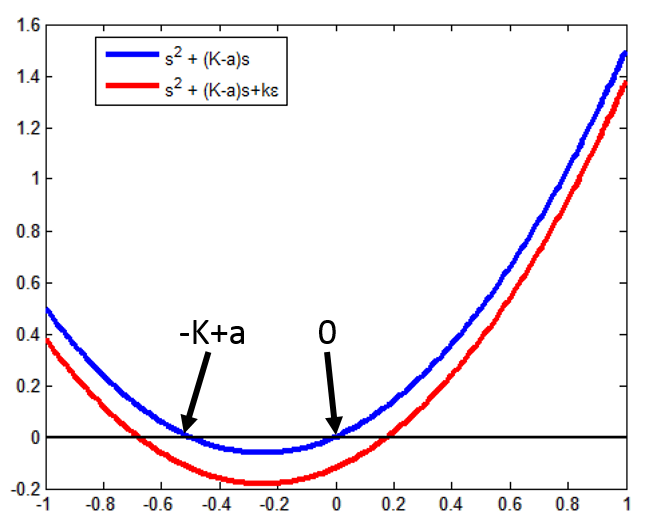
\includegraphics[width=1.2\linewidth]{robustness-example}
			\label{fig:robustness-example}
		\end{figure}
	\end{minipage}
\end{frame}


\begin{frame}
	\frametitle{Example 3: Robustness of steady-state error}
	\begin{itemize}
		\item The steady state error is defined as follows:
		\begin{align*}
			\lim\limits_{t \rightarrow \infty} e(t)
			&= \lim\limits_{t \rightarrow \infty} (r(t) - y(t)) \\
			&= \lim\limits_{s \rightarrow 0} s(R(s) - Y(s)) &\text{(final value theorem)}
		\end{align*}
		
		\item A very small steady state error (preferably zero) indicates that the controller tracks the reference very well
		
		\item For the open loop system with a step reference
		\begin{align*}
			e_{ol}(\infty) &= \lim\limits_{s \rightarrow 0}
			s(1 - C(s)P(s))R(s) = 1 - C(0)P(0)
		\end{align*}
		\begin{itemize}
			\item So the open loop controller can be free of a steady state error (for a step reference $\epsilon(t)$) by calibrating the controller such that $C(0)P(0)=1$
			\item $\Rightarrow$ a precise calibration of the DC gain
		\end{itemize}
	\end{itemize}
	
\end{frame}


\begin{frame}
	\frametitle{Example 3: Steady state error}
	\begin{itemize}
		\item Closed loop system:
		\begin{flalign*}
			e_{cl}(\infty) &= \lim\limits_{s \rightarrow 0} s\left(1 - \frac{C(s)P(s)}{1+C(s)P(s)}\right)R(s) \\
			&= \lim\limits_{s \rightarrow 0} \frac{s}{1 + C(s)P(s)}R(s) = \frac{1}{1+C(0)P(0)}
		\end{flalign*}
		\begin{itemize}
			\item The steady state error is small if $C(0)P(0)$ is very large
			\item Again, calibrating the DC gain
			\item The difference is that here we only need a large gain, which is far less demanding than having to make it equal to 1
		\end{itemize}
	\end{itemize}
\end{frame}

\begin{frame}
	\frametitle{An open loop controller is not robust}
	\begin{itemize}
		\item We can now show how this results in a great advantage of the closed loop strategy over the open loop strategy:
		\begin{itemize}
			\item If $P$ changes slightly (for instance due to a factor that has not been taken up into the model) to $P+\Delta P$
			\item Then making $e_{ol}(\infty)$ small would require to calibrate anew
			\item Whereas $e_{cl} (\infty)$ would remain small, as long as $(P(0)+\Delta P(0))C(0)$ remains large
			
		\end{itemize}
		\item Hence an open loop controller can't control the output \textbf{robustly} against changes in $P$
	\end{itemize}
\end{frame}

\subsection[Types of systems and SS-error]{Types of systems and Steady State Error}

\begin{frame}
	\frametitle{Type of a system}
	\begin{itemize}
		\item For a step reference $r(t) = A \epsilon (t)$ $\Rightarrow R(s) = \frac{A}{s}$
		\[e_{cl}(\infty) = \frac{A}{1+C(0)P(0)} \]
		So $e_{cl}(\infty) = 0$ if C(s)P(s) has a least one pole in zero ($C(0)P(0) \rightarrow \infty$)
		\item For a ramp reference function $r(t) = At \, \Rightarrow R(s) = \frac{A}{s^2}$, we have
		\begin{flalign*}
			e_{cl}(\infty) = \lim\limits_{s \rightarrow 0} \frac{s}{1+C(s)P(s)} \frac{A}{s^2}
		\end{flalign*}
		So $e_{cl}(\infty) = 0$ if $C(s)P(s)$ has at least two poles in zero. $\left(\lim\limits_{s\rightarrow 0} sC(s)P(s) = \infty\right)$
	\end{itemize}
\end{frame}

\begin{frame}
	\frametitle{Type of a system}
	\begin{itemize}
		\item The type of a system is determined by the number of poles $P(s)C(s)$ has in zero, and hence it is linked to what type of references it can track perfectly
		\item Write $P(s)C(s)$ as $\frac{K \prod_{k=1}^{m} (s-z_k)}{s^l \prod_{k=1}^{n-l} (s-p_k)}$ with $l$ the amount of poles in zero
		\item We say this system is of type $l$
		\begin{itemize}
			\item It will be able to track references of shape $At^0 \epsilon(t)$ up to $At^{(l - 1)} \epsilon(t)$ perfectly (for $t\rightarrow \infty$, $\lim\limits_{t \rightarrow \infty} e_{cl}(t) = 0$)
			\item A reference of shape $At^l \epsilon(t)$ will be missed by a finite factor (for $t\rightarrow \infty$, $\lim\limits_{t \rightarrow \infty} e_{cl}(t) = C$)
			\item A reference of shape $At^{l+...} \epsilon(t)$ will be missed by infinity (for $t\rightarrow \infty$, $\lim\limits_{t \rightarrow \infty} e_{cl}(t) = \infty$)
		\end{itemize}
	\end{itemize}
\end{frame}

\begin{frame}
	\frametitle{Example of a type 0 system}
	\begin{itemize}
		\item Step reference $r(t) = A \epsilon (t) \Rightarrow R(s) = \frac{A}{s}$
		\begin{flalign*}
			e_{cl}(\infty) &= \lim\limits_{s \rightarrow 0} \frac{s}{1 + C(s)P(s)} \frac{A}{s} \\
			&= \lim\limits_{s \rightarrow 0} \frac{A}{1 +  \frac{K \prod_{k=1}^{m} (-z_k)}{\prod_{k=1}^{n-l} (-p_k)}}
			= \frac{A}{1 + K_p}
		\end{flalign*}
		with $K_p$ the static position constant
		\item Ramp reference $r(t) = At \epsilon (t) \Rightarrow R(s) = \frac{A}{s^2}$
		\begin{flalign*}
			e_{cl}(\infty) &= \lim\limits_{s \rightarrow 0} \frac{s}{1+C(s)P(s)} \frac{A}{s^2} \\
			&= \lim\limits_{s \rightarrow 0} \frac{1}{1 + \frac{K \prod_{k=1}^{m} (-z_k)}{\prod_{k=1}^{n-l} (-p_k)}} = \infty
		\end{flalign*}
	\end{itemize}
\end{frame}	

\begin{frame}
	\frametitle{Steady state errors - type of a system}
	\begin{itemize}
		\item With:
			\begin{tabbing}
			$K_p = \lim\limits_{s \rightarrow 0} P(s)C(s)$ 
			\hspace{2em} \= $K_p = $ Static position constant \\
			$K_v = \lim\limits_{s \rightarrow 0}s P(s)C(s)$ \> $K_v = $ Static velocity constant \\
			$K_a = \lim\limits_{s \rightarrow 0}s^2 P(s)C(s)$ \> $K_a = $ Static acceleration constant
			\end{tabbing}
		\item And the respective steady state errors for different system types are:
		\begin{tabular}{|l|c|c|c|}
			\hline \textbf{Type} $\mathbf{l}$ & \textbf{Step} $\mathbf{A \boldsymbol{\epsilon} (t)}$ & \textbf{Ramp} $\mathbf{At \boldsymbol{\epsilon} (t)}$ & \textbf{Parabola} $\mathbf{\frac{At^2 \boldsymbol{\epsilon} (t)}{2}}$ \\ 
			\hline \textbf{0} & $\frac{A}{1 + K_p}$ & $\infty$ & $\infty$ \\ 
			\hline \textbf{1} & 0 & $\frac{A}{K_v}$ & $\infty$ \\ 
			\hline \textbf{2} & 0 & 0 & $\frac{A}{K_a}$ \\ 
			\hline 
		\end{tabular} 
	\end{itemize}
\end{frame}


\subsection[Noise- and disturbance rejection]{Noise- and disturbance rejection}

\begin{frame}
	\frametitle{Noise rejection and disturbance rejection}
	\begin{itemize}
		\item Both refer to rejection of the input $D$ but are not the same
		\item Measurement noise is often modelled by white noise. (High frequency signal)
		\item Disturbances are actual changes to the state of the system
	\end{itemize}
\begin{figure}
\centering
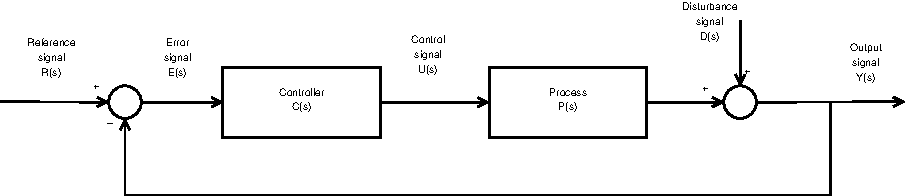
\includegraphics[width=0.7\linewidth]{Closed-Loop}
\label{fig:Closed-Loop3}
\end{figure}
\end{frame}


\begin{frame}
	\frametitle{Noise versus Disturbances}
	\begin{itemize}
		\item Cruise control: \\
		Measurement errors on the speed are noise \\
		A change in slope is a disturbance
	\end{itemize}
	\begin{figure}
\centering
\includegraphics[width=0.7\linewidth]{"cruise control"}
\label{fig:cruisecontrol}
\end{figure}
\end{frame}

\begin{frame}
	\frametitle{Noise versus Disturbances}
	\begin{itemize}
		\item Remember from the start of the lecture
		\begin{align*}
			Y(s) = \frac{P(s)C(s)}{1+P(s)C(s)}R(s) + \frac{1}{1+P(s)C(s)}D(s)
		\end{align*}
		\item Choosing $T(s)=\frac{1}{1+P(s)C(s)}$ sufficiently small results in the rejection of $D$. This can be achieved by choosing $C(s)$ sufficiently high
	\end{itemize}
	\begin{figure}
\centering
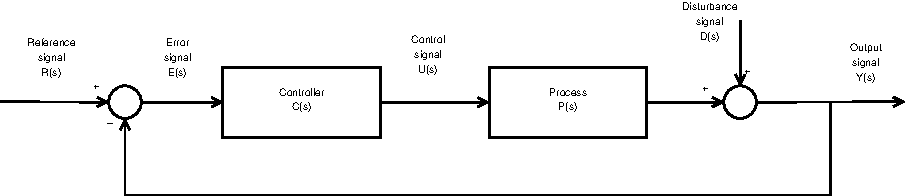
\includegraphics[width=0.7\linewidth]{Closed-Loop}
\label{fig:Closed-Loop4}
\end{figure}
\end{frame}


\begin{frame}
	\frametitle{Disturbance vs noise}
	\begin{itemize}
		\item But what happens to measurement noise
		\begin{itemize}
			\item The amplified measurement noise will be applied to the input of the plant.
			\item In reality measurement noise requires no control actions. Good noise rejection means that the controller ignores this noise.
		\end{itemize}
	\end{itemize}
	\begin{figure}
\centering
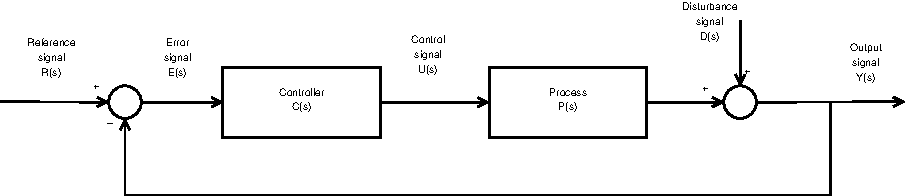
\includegraphics[width=0.7\linewidth]{Closed-Loop}
\label{fig:Closed-Loop5}
\end{figure}
\end{frame}


\begin{frame}
	\frametitle{Disturbance versus noise rejection}
	\begin{itemize}
		\item Good disturbance rejection requires fast action to bring the state back to the desired state
		\item Good noise rejection requires that measurement noise will be ignored
		\item Note that a controller can not see the difference between measurement noise and disturbances. Slow controllers will be less sensitive to measurement noise. Fast system will have better disturbance rejection
	\end{itemize}
\end{frame}

\newcommand{\specialcell}[2][c]{%
	\begin{tabular}[#1]{@{}c@{}}#2\end{tabular}}
\begin{frame}
	\frametitle{Classical trade-offs in control theory}
	\begin{tabular}{ll}
		\specialcell[]{\textbf{Slow Controllers:} \\ Not sensitive to noise \\ Small control inputs} & \specialcell[]{\textbf{Fast controllers:} \\ Good disturbance rejection \\ Fast tracking}\\ 
		\specialcell[]{\textbf{Robust controllers:} \\ Model errors will not\\ affect the behaviour of\\ the system strongly} & \specialcell[]{\textbf{Aggresive controllers:} \\ Exchanges robustness for \\ better performance}  \\ 
	\end{tabular}
\end{frame}